\chapter{Method Details}

\section{Record Linkage}
\label{sec:record-linkage-appendix}

The Jaro-Winkler formula is defined in two steps. First, The Jaro distance, $d_j $, is defined as:

% good code-based illustration at: http://www.gettingcirrius.com/2011/01/calculating-similarity-part-2-jaccard.html

\begin{equation}
  d_j = \left\{
  \begin{array}{l l}
    0 & \text{if }m = 0 \\ 
    \frac{1}{3}\left(\frac{m}{|s_1|} + \frac{m}{|s_2|} + \frac{m-t}{m}\right) & \text{otherwise} \end{array} \right.
\end{equation}

Where:

m = number of matching patterns
t = number of transposed characters
|s1| = length of first string
|s2| = length of second string

Two characters are considered matching when they are no further apart than:
\begin{equation}
  \left\lfloor\frac{\max(|s_1|,|s_2|)}{2}\right\rfloor-1
\end{equation}

The second component, added by Winkler, preferentially weights strings which match from the beginning, set by the prefix length $ l $.  Thus, the Jaro-Winkler distance is defined:

\begin{equation}
  d_w = d_j + (\ell p (1 - d_j))
\end{equation}

Where $ p $ is a constant scaling factor to adjust for the strength of common prefixes. In its usage here, $ p = 0.1 $ and $ l = 4 $.


\section{Observation Filtering}
% XXX oliver: Cool, power-law, but how exactly do you use this to filter?  Is there more than just screening by the theoretical maximum?
As in many large datasets, the distribution of observations per ship follows an approximate power-law distribution. Using the raw number of observations received in our 15 month window provides a simple filter. The peak in the kernel density estimation (Figure \ref{fig:obs-per-vessel-log}) is seen around $10^4$ observations, with a clear drop-off after $10^5$, which is consistent with the theoretical maximum (one observation in every sample) of about $6.8 \times 10^5$.
\begin{figure}[htbp]
  \centering
  \includegraphics[width=120mm]{figures/obs-per-vessel-log-qplot.pdf}
  \caption[Observations per vessel]{Observations per vessel, kernel density estimation.}
  \label{fig:obs-per-vessel-log}
\end{figure}

\section{Movement Modeling}
\label{sec:movement-modeling-appendix}

% XXX From Jano: provide more detail on what actually was done. Code, whatever, fine -- but include details. It can be in an appendix, but need to include information like cell size, processing techniques, and other details of what the heck you actually did. [Move some stuff from the methods into this appendix].
% XXX copy and paste job, include details here.... tools used? DETAILED APPROACH.

Each vessel track was rasterized to both an 90 arcsecond grid (\textasciitilde{}5.5km at the equator) and an equal area grid in the Hobo Dyer projection (Figure \ref{fig:eu-cargo-density}). The latter case assures that the density function is computed on grid cells representing the same area for each cell, unlike the geographic grid where area varies by latitude. A vessel is counted only once for each cell it passes through, as the focus here on overall movement patterns, and this criteria helps de-emphasize vessels with limited movement. Each raster vessel track was combined using simple map algebra to produce density maps for both the AIS and VOS data, for each of our vessel classes. % XXX Oliver: A passing cargo ship is comparable to a ferry crisscrossing the same spot continuously every day?  Not that you should do this, but somebody might wonder.

% XXX gdal_rasterize did the rasterization step

% gdal_add, custom python code combined the results

% paralellized in Python.

% Bresenham's line algorithm used for rasterizing the tracks. Only counted a ship moving through a single cell once to get movement patterns v. dockage

% XXX built spatial indexes and reordered the data on disk to match for performance.

% Store the raw observations in a spatial database (PostGIS), use parallelized code to quickly aggregate the results.

\chapter{Tables}

\begin{table}[htbp]
  \caption[AIS broadcast attributes]{AIS broadcast attributes. Update frequency depends on ship speed, but varies between a minimum of a record every 2 seconds for quickly moving vessels, to once per 3 minutes for moored vessels. Additional attributes are available, but infrequently used.}
  \begin{tabular}{lr}
    \hline
    Attribute & Accuracy \\
    \hline
    Location (fixed from GPS signal) & $\simeq$10 meter accuracy) \\
    Timestamp (on broadcast) & $\simeq$100 ms \textit{transmission \& processing}\\
    Name \\
    Call Sign \\
    Maritime Mobile Service Identity (MMSI) \\
    Heading \\
    Speed \\
    Destination & \textit{often incorrect}
  \end{tabular}
  \label{table:ais-broadcast-attributes}
\end{table}

% table describing the record linkage technique used for each data source
% SOURCE: record-linkage/FRIL/config/*.xml
\begin{table}[htbp]
  \caption[Ship record linkage methods]{Ship record linkage methods used.}
  \ssp
  \begin{tabular}{rrrlrr}
    \hline
    Source $A$ & Source $B$ & acceptance level & column & distance metric & weight \\
    \hline
     DS & ITU & 92 & callsign & Jaro-Winkler\textsuperscript{1} & 50 \\
        &     &    & MMSI & equal & 40 \\
        &     &    & name & Jaro-Winkler & 40 \\
     DS &  VT & 85 & callsign & Jaro-Winkler & 60 \\
        &     &    & IMO & Jaro-Winkler & 20 \\
        &     &    & name & Jaro-Winkler & 20 \\
    FCC & ITU & 85 & callsign & Jaro-Winkler & 95 \\
        &     &    & name & Jaro-Winkler & 5 \\
    FCC &  VT & 95 & callsign & Jaro-Winkler & 66 \\
        &     &    & name & Jaro-Winkler & 5 \\
        &     &    & MMSI & Jaro-Winkler & 24 \\
        &     &    & length & equal & 5 \\
     VT & ITU & 80 & callsign & Jaro-Winkler & 20 \\
        &     &    & MMSI & Edit Distance & 30 \\
        &     &    & name & Jaro-Winkler & 10 \\
        &     &    & IMO & Jaro-Winkler & 40 \\
     DS & FCC & 95 & callsign & equal & 99 \\
        &     &    & name & Jaro-Winkler& 1 \\
  \end{tabular}
  \\
  \textsuperscript{1} Jaro-Winkler distance \citep{winkler1990string}: length $l = 4$ and scaling factor $p = 0.1$
  \label{table:ships-record-linkage-methods}
\end{table}


% had this as a list, also some hackery with unnesting class data:
% select distinct(trim(both from unnest(class))), count(*) from clean.ships where validation_class = 'tanker' and validation_score > 0 and obs_count > 0 GROUP BY class ORDER BY btrim DESC;ships=# select distinct(trim(both from unnest(class))), count(*) from clean.ships where validation_class = 'tanker' and validation_score > 0 and obs_count > 0 GROUP BY class ORDER BY btrim DESC;
\begin{longtable}{l|l|l}

\hline \multicolumn{1}{|c|}{\textbf{Type}} & \multicolumn{1}{c|}{\textbf{Sub-type}} & \multicolumn{1}{c|}{\textbf{Vessels}} \\ \hline 
\endfirsthead
%\multicolumn{3}{c}%
%{{\bfseries \tablename\ \thetable{} -- continued from previous page}} \\
\hline \multicolumn{1}{|c|}{\textbf{Type}} &
\multicolumn{1}{c|}{\textbf{Sub-type}} &
\multicolumn{1}{c|}{\textbf{Vessels}} \\ \hline 
\endhead

%\hline \multicolumn{3}{|r|}{{Continued on next page}} \\ \hline
\endfoot
    cargo & cargo ship & 30355 \\
          & merchant & 2919 \\
          & bulk carrier & 1338 \\
          & container ship & 669 \\
          & general cargo & 608 \\
          & vehicle carrier & 56 \\
    tanker & tankship & 10460 \\
           & tanker   & 8731 \\
           & oil tanker & 1312 \\
           & liquefied gas carrier & 112 \\
           & chemical carrier & 39 \\
    other & merchant & 17460 \\
          & other ship & 9421 \\
          & unspecified & 4580 \\
          & motor boat & 4231 \\
          & inland waterways & 3825 \\
          & sloop & 2799 \\
          & reserved for future use & 2164 \\
          & all other activities & 1345 \\
          & reserved for regional use & 712 \\
  support & pusher/tug & 4392 \\
          & tug & 7885 \\
          & towing vessel & 2747 \\
          & supply vessel & 1501 \\
          & service vessels & 1388 \\
          & trawler & 1056 \\
          & dredger & 995 \\
          & vessel engaged in dredging or underwater operation & 776 \\
          & pilot vessel & 685 \\
  pleasure & pleasure/leisure & 22013 \\
           & pleasure & 14573 \\
           & pleasure craft & 7290 \\
           & sailing vessel & 5527 \\
           & yacht & 8214 \\
  fishing & fishing vessel & 11110 \\
          & fishing boat & 8454 \\
          & fishing industry & 5767 \\
          & fishing & 3213 \\
  passenger & passenger ship & 6478 \\
            & ferry & 704 \\
  high-speed & high-speed craft & 658 \\
             & high speed craft & 520 \\
  authority & sar-vessel & 699 \\
            & search and rescue vessel & 609 \\
            & rescue vessel & 102 \\
  \caption[Detailed ship classes]{Detailed ship classes, derived from observations.}
  \label{table:ship-class-breakdown}
\end{longtable}

\chapter{Software}
\label{sec:software}

% include SOME python code here -- our AIS parser, what else?
% steps: download AIS
% parse AIS
% insert AIS into DB, formalize
% download & parse ship databases

This work would not have been possible without extensive contributions from others in the form of software, both commercial and open source. An overview of the software used in the project is provided, and the code produced is available at https://github.com/scw/ais-kml-parser. 

To store the raw observations, \textsf{SQLite} was used for rapid development, but the bulk of the observations were stored in the object-relational database \textsf{PostgreSQL}, where the majority of the analysis was carried out using either native SQL or with the spatial extension \textsf{PostGIS}. The \textsf{GDAL} library was used extensively for transforming both raster and vector data. Record linkage was performed using \textsf{FRIL}, with some record linkage integrated into the database using \textsf{pg\_similarity}, and in \textsf{Python} using the \textsf{jellyfish} module. Integration and data processing used \textsf{Python}, which combines a wide base of environments within a single language. \textsf{R} was used to perform statistical analyses and summarize results. \textsf{GRASS} was used to compute model outputs and spatial statistics, and maps were produced in \textsf{ArcGIS} and \textsf{Quantum GIS}.

\begin{table}[htbp]
  \caption[Software used]{Software used, version details}
  \ssp
  \begin{tabular}{rr}
    \hline
    Software package & version \\
    \hline
     \textsf{ArcGIS} & 10.1 \\
     \textsf{Bash} & 4.2.24 \\ 
     \textsf{FRIL} & 2.1.5 \\
     \textsf{GDAL} & 1.8.0 \\
                 " & 1.9.1 \\
                 " & 1.9.2 \\
     \textsf{Git} & 1.7.9.5 \\
     \textsf{GRASS} & 6.4 \\
                  " & 7.0 \\
     \textsf{pg\_similarity} & 0.0.19 \\
     \textsf{PostGIS} & 1.5.3 \\
                    " & 2.0.1 \\
     \textsf{PostgreSQL} & 8.4.14 \\
                      "  & 9.2.1 \\
     \textsf{Python} & 2.6 \\
                   " & 2.7.2 \\
     \textsf{Quantum GIS} & 1.8 \\
     \textsf{R} & 2.14 \\
              " & 2.15 \\
     \textsf{SQLite} & 3.7.9 \\
  \end{tabular}
  \label{table:software-used-versions}
\end{table}

R was used for calculations, validation, and statistics, the following packages were utilized:
\begin{itemize}
  \item foreign
  \item geosphere
  \item ggplot2
  \item maptools
  \item plotrix
  \item raster
  \item RPostgreSQL
  \item rgdal
  \item rgeos
  \item sm
  \item sp
\end{itemize}

Python was used extensively, the external libraries used included:
\begin{itemize}
  \item BeautifulSoup
  \item gdal
  \item geographiclib
  \item geojson
  \item geopy
  \item grass
  \item jellyfish
  \item numpy
  \item ogr
  \item psycopg2
  \item requests
\end{itemize}

\chapter{Figures}
\label{sec:figures}

\begin{figure}[htbp]
  \centering
  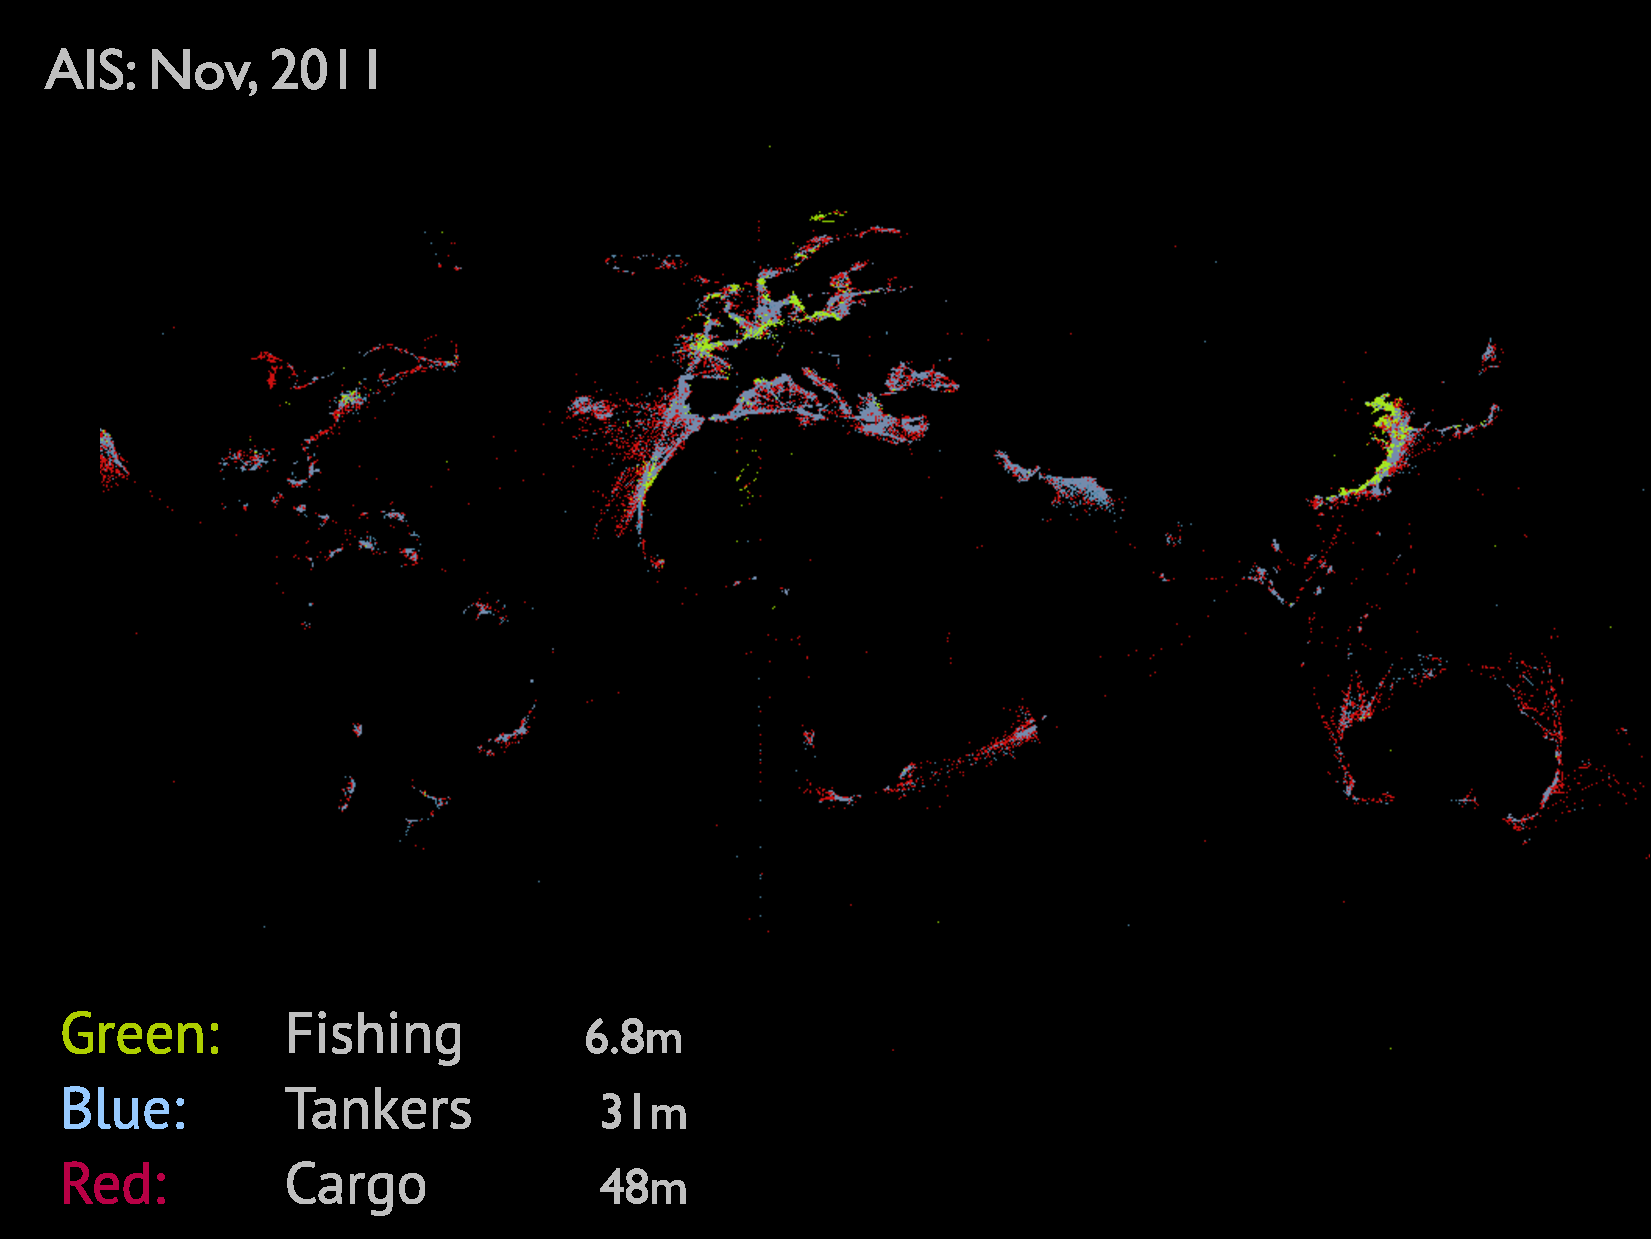
\includegraphics[width=160mm]{figures/ais-nov-2011.pdf}
  \caption[AIS observations, November 2011]{Raw AIS observations, November 2011. Note the observations located in the Hoggar Mountains in Algeria.}
  \label{fig:ais-obs-nov-2011}
\end{figure}

% show our image of invalid 'on land' ships in the harbor of long beach?
\begin{figure}[htbp]
  \centering
  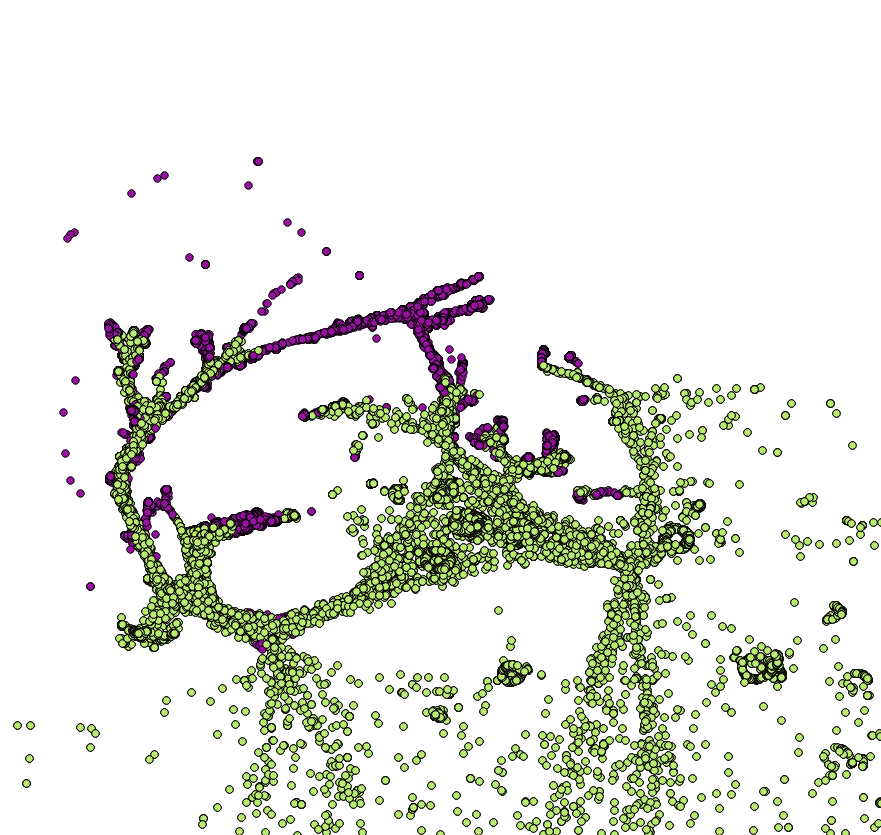
\includegraphics[width=140mm]{figures/example-long-beach-harbor-validation.png}
  \caption[Long beach harbor, validation example]{Long Beach Harbor, California. Points shown here in purple are 'on land', but most of these on-land observations are actually parts of the harbor.} % XXX Oliver: a little context here?
  \label{fig:longbeach-validation}
\end{figure}


\begin{figure}[htbp]
  \centering
  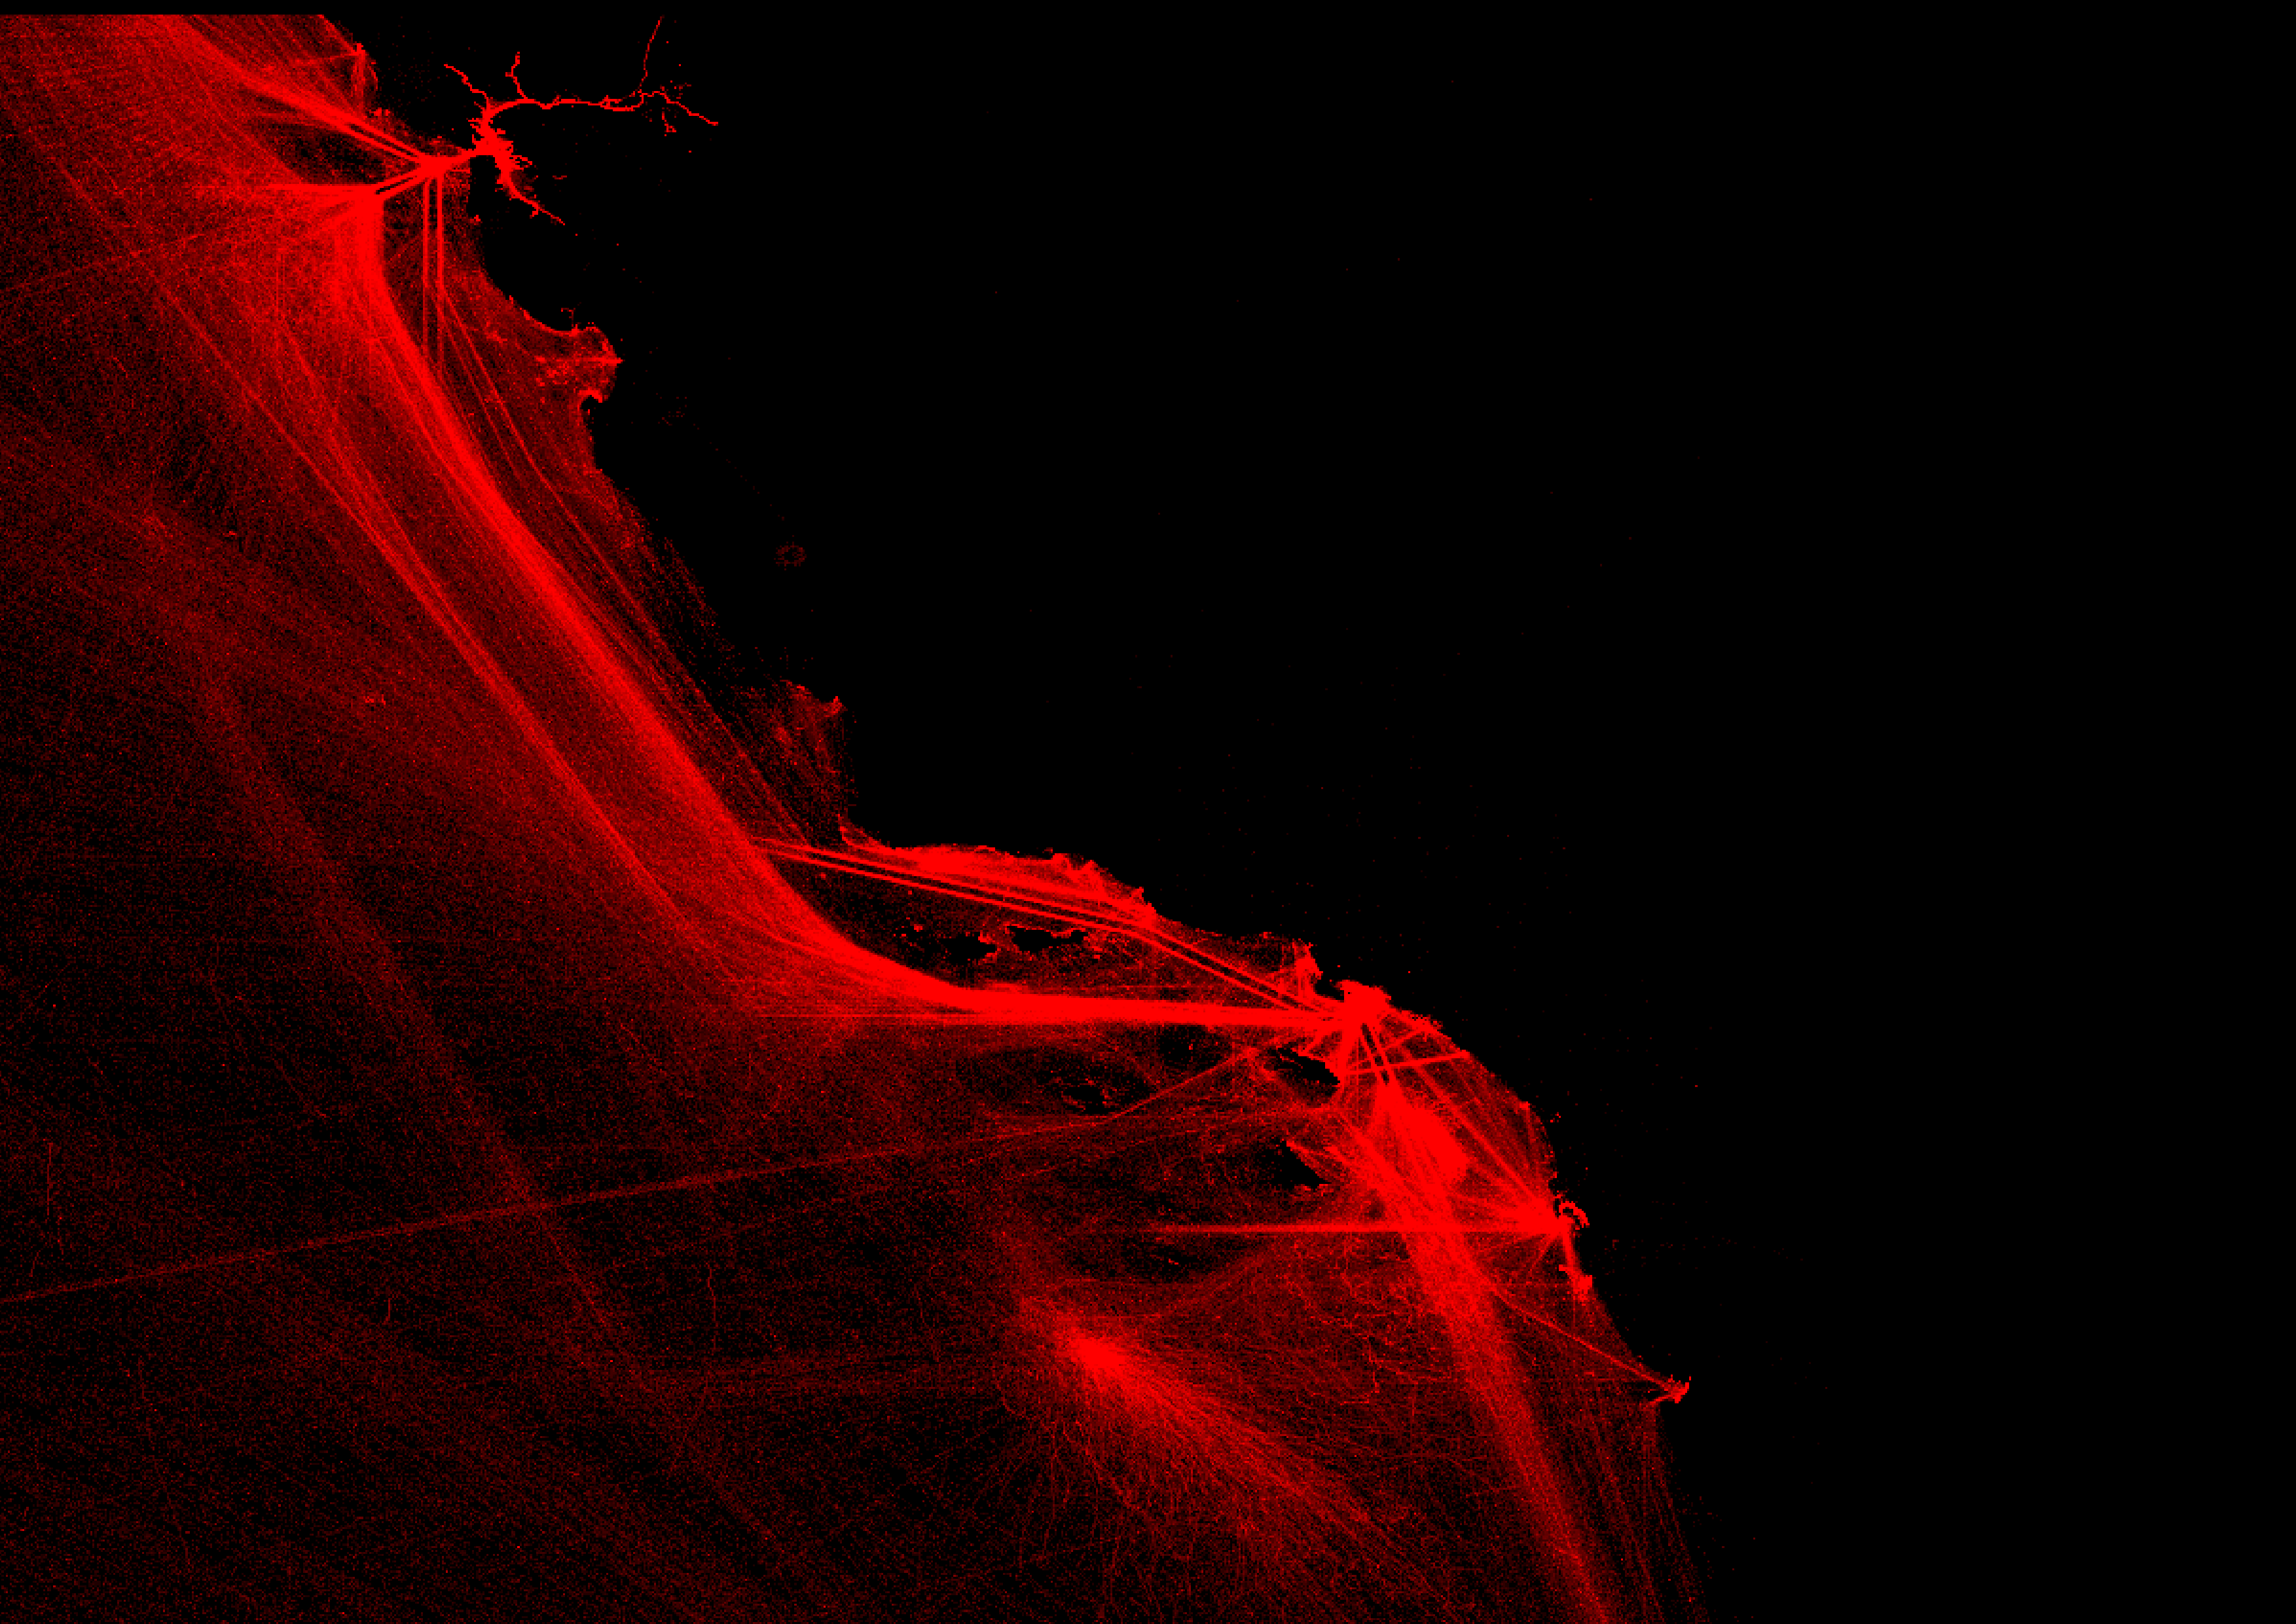
\includegraphics[width=140mm]{figures/cargo_density.png}
  \caption[AIS observations, Southern California Bight]{AIS observations, Southern California Bight. Nov 2010--Dec 2011. Note the ballast water exchange point lower left.}
  \label{fig:cal-cargo}
\end{figure}

\begin{figure}[htbp]
  \centering
  \includegraphics[width=160mm]{figures/ais-and-ports-cea.pdf}
  \caption[AIS coverage]{Approximate AIS coverage (green), global ports (red).}
  \label{fig:ais-coverage}
\end{figure}

\begin{figure}[htbp]
  \centering
  \includegraphics[width=160mm]{figures/cia-lanes-small-cropped.png}
  \caption[CIA "World Shipping Lanes"]{"World Shipping Lanes" map produced by the Central Intelligence Agency, 1973.}
  \label{fig:cia-shipping-map}
\end{figure}


